\documentclass[11pt,a4paper]{article}
\usepackage[margin=2.6cm]{geometry}
\usepackage[T1]{fontenc}
\usepackage{lmodern}
\usepackage[letterspace=180]{microtype}
\usepackage{booktabs}
\usepackage{amsmath}
\usepackage{parskip}
\usepackage{xcolor}
\usepackage{tikz}
\usetikzlibrary{shapes.geometric,arrows.meta,positioning}
\usepackage[most]{tcolorbox}
\usepackage{titlesec}
\usepackage{caption}
\usepackage{graphicx}

\definecolor{bcnavy}{RGB}{24,38,68}
\definecolor{bcgold}{RGB}{198,160,74}
\definecolor{bcteal}{RGB}{23,110,120}
\definecolor{bcgrey}{RGB}{95,95,95}
\definecolor{bcred}{RGB}{160,60,50}

\titleformat{\section}{\bfseries\large\color{bcnavy}}{\thesection.}{0.6em}{}
\titleformat{\subsection}{\bfseries\color{bcteal}}{}{0em}{}
\captionsetup{font={footnotesize},labelformat=empty,textfont={color=bcgrey}}
\newcommand{\tabnote}[1]{\begin{center}\begin{minipage}{0.92\textwidth}
  \footnotesize\color{bcgrey}#1\end{minipage}\end{center}}
\newcommand{\pass}{{\color{bcteal}\textbf{pass}}}
\newcommand{\fail}{{\color{bcred}\textbf{fail}}}
\newcommand{\flagg}{{\color{bcgold}\textbf{flag}}}

\begin{document}

% ---------------------------------------------------------------- cover
\begin{titlepage}
\centering
\vspace*{3.2cm}

\includegraphics[width=5cm]{bc_logo.pdf}

\vspace{1.6cm}
{\color{bcnavy}\rule{7cm}{0.6pt}}

\vspace{0.9cm}
{\LARGE\bfseries\color{bcnavy} Book Admission Gates\par}
\vspace{0.35cm}
{\large\color{bcnavy} The criteria a stock must clear to enter the nine-name book,\\
and the standing disciplines behind them\par}

\vspace{0.9cm}
{\color{bcgold}\rule{7cm}{1.0pt}}

\vspace{1.5cm}
{\bfseries Bayesian Capital}\\[0.2cm]
{\color{bcgrey} Systematic Trading Research}\\[0.9cm]
{\itshape\color{bcgrey} Internal document --- strictly confidential}\\[0.3cm]
{\color{bcgrey} 10 August 2026 --- revised 14 August 2026 (MRVL admission)}
\vfill
\end{titlepage}

% ---------------------------------------------------------------- header
\begin{center}
{\Large\bfseries\color{bcnavy} Book Admission Gates}\\[0.15cm]
{\color{bcnavy} The criteria a stock must clear to enter the book, and the
standing disciplines behind them}\\[0.25cm]
{\small\color{bcgrey} Bayesian Capital --- Systematic Trading Research
\;$\bullet$\; current book: TSM $\cdot$ VRT $\cdot$ VST $\cdot$ RKLB $\cdot$ MU
$\cdot$ GM $\cdot$ VLO $\cdot$ CF $\cdot$ MRVL \;$\bullet$\; all figures on verified fills}
\end{center}
\vspace{0.1cm}
{\color{bcnavy}\hrule height 0.8pt}
\vspace{0.5cm}

\section{Purpose}

Admission to the book is the decision that moves realised returns more than any
parameter, and it is the decision most exposed to wishful evidence. This document
fixes the gates a candidate must clear, in order, so that every future admission
--- and every decline --- is the same decision made the same way. The gates codify
what the August 2026 reviews actually did: they admit GM, VLO and CF, then MRVL;
they decline NVDA, AVGO, TSLA, AMD, SMCI and CEG; and they flag VST. A candidate that cannot be pushed through
every gate does not trade.

\section{Two classes, two return requirements}

Every candidate is classified before it is scored, using its share-return beta to
the AI factor (the equal-weight daily return of TSM, VRT, VST and MU) and the
correlation of its verified strategy returns to the current book:

\begin{center}
\begin{tabular}{lccc}
\toprule
class & AI-factor beta & book correlation & \textbf{planned return gate} \\
\midrule
\textbf{AI-related}   & $> 0.20$   & any        & $\boldsymbol{\geq 50\%}$/yr \\
\textbf{Uncorrelated} & $\leq 0.20$ & $\leq 0.25$ & $\boldsymbol{\geq 30\%}$/yr \\
\bottomrule
\end{tabular}
\end{center}

\tabnote{Classification is conservative: a name that fails either uncorrelated
test carries the AI gate. The planned return is the \emph{planning figure} ---
unseen-window median, or through-cycle verified less the measured out-of-sample
haircut --- never a raw fitted or full-sample number.}

The asymmetry is deliberate. An AI-related name adds to the book's dominant risk,
so it must decisively out-earn what it concentrates: the book's AI names plan at
55--156\%, and a candidate below 50\% dilutes return while adding beta --- the
worst trade available. An uncorrelated name earns its place differently: at beta
$\leq 0.2$ its risk is additive-diversifying, it cuts the book's stress loss and
drawdown, and 30\% is the level at which that insurance is bought for an
acceptable spread against the book's $\approx$65\% planning average. GM, VLO and
CF were admitted at 33--41\% planned on exactly this arithmetic, taking the
Jan--Apr 2025 stress loss from $-18.7\%$ to $-11.8\%$.

\section{The gate sequence}

\begin{center}
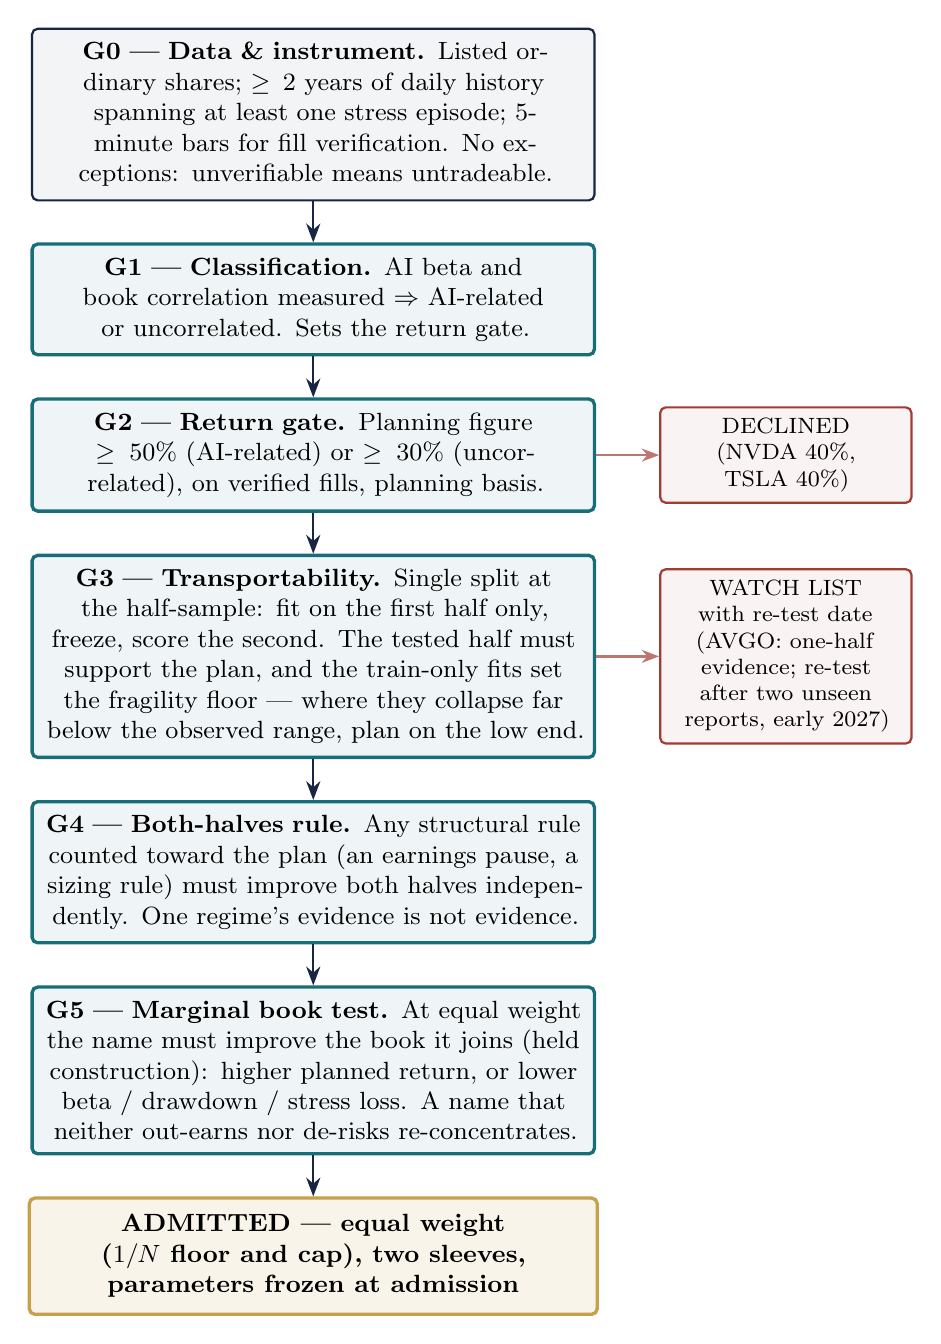
\begin{tikzpicture}[
  node distance=5.2mm and 8mm,
  box/.style={rectangle, rounded corners=2pt, draw=bcnavy, thick, fill=bcnavy!5,
    text width=0.56\textwidth, align=center, inner sep=5pt, font=\small},
  gate/.style={rectangle, rounded corners=2pt, draw=bcteal, very thick, fill=bcteal!7,
    text width=0.56\textwidth, align=center, inner sep=5pt, font=\small},
  declined/.style={rectangle, rounded corners=2pt, draw=bcred, thick, fill=bcred!6,
    text width=0.24\textwidth, align=center, inner sep=4pt, font=\footnotesize},
  final/.style={rectangle, rounded corners=2pt, draw=bcgold, very thick, fill=bcgold!12,
    text width=0.56\textwidth, align=center, inner sep=6pt, font=\small\bfseries},
  arr/.style={-{Stealth[length=2.4mm]}, thick, bcnavy},
  rej/.style={-{Stealth[length=2.2mm]}, thick, bcred!70}]

\node[box] (g0) {\textbf{G0 — Data \& instrument.} Listed ordinary shares; $\geq 2$
  years of daily history spanning at least one stress episode; 5-minute bars for
  fill verification. No exceptions: unverifiable means untradeable.};
\node[gate, below=of g0] (g1) {\textbf{G1 — Classification.} AI beta and book
  correlation measured $\Rightarrow$ AI-related or uncorrelated. Sets the return
  gate.};
\node[gate, below=of g1] (g2) {\textbf{G2 — Return gate.} Planning figure
  $\geq 50\%$ (AI-related) or $\geq 30\%$ (uncorrelated), on verified fills,
  planning basis.};
\node[gate, below=of g2] (g3) {\textbf{G3 — Transportability.} Single split at the
  half-sample: fit on the first half only, freeze, score the second. The tested
  half must support the plan, and the train-only fits set the fragility floor ---
  where they collapse far below the observed range, plan on the low end.};
\node[gate, below=of g3] (g4) {\textbf{G4 — Both-halves rule.} Any structural rule
  counted toward the plan (an earnings pause, a sizing rule) must improve both
  halves independently. One regime's evidence is not evidence.};
\node[gate, below=of g4] (g5) {\textbf{G5 — Marginal book test.} At equal weight
  the name must improve the book it joins (held construction): higher planned
  return, or lower beta / drawdown / stress loss. A name that neither out-earns
  nor de-risks re-concentrates.};
\node[final, below=of g5] (adm) {ADMITTED — equal weight ($1/N$ floor and cap),
  two sleeves, parameters frozen at admission};
\node[declined, right=of g2] (w2) {\footnotesize DECLINED\\ (NVDA 40\%, TSLA 40\%)};
\node[declined, right=of g3] (w3) {\footnotesize WATCH LIST with re-test date\\ (AVGO:
  one-half evidence; re-test after two unseen reports, early 2027)};

\draw[arr] (g0) -- (g1);
\draw[arr] (g1) -- (g2);
\draw[arr] (g2) -- (g3);
\draw[arr] (g3) -- (g4);
\draw[arr] (g4) -- (g5);
\draw[arr] (g5) -- (adm);
\draw[rej] (g2) -- (w2);
\draw[rej] (g3) -- (w3);
\end{tikzpicture}
\end{center}
\tabnote{A failed gate ends the assessment. A near-miss on selected or one-half
evidence goes to the watch list with a defined re-test date on data that did not
exist when the case was made --- never to a re-fit.}

\section{The current book against the gates}

\begin{center}
\small
\begin{tabular}{llrrrcccc}
\toprule
 & class & plan & AI $\beta$ & corr & G2 gate & G2 & G3 & note \\
\midrule
RKLB & AI    & 156\% & 0.79 & 0.94 & 50\% & \pass & \flagg & fragility floor 12\%: plan low end \\
VRT  & AI    &  65\% & 1.19 & 0.48 & 50\% & \pass & \pass & \\
MU   & AI    &  61\% & 1.14 & 0.59 & 50\% & \pass & \pass & P3 earnings pause adopted (G4 \pass) \\
TSM  & AI    &  55\% & 0.69 & 0.47 & 50\% & \pass & \pass & \\
MRVL & AI    &  78\% & 0.95 & 0.22 & 50\% & \pass & \pass & only name whose train-only fits clear the gate outright \\
VST  & AI    &  50\% & 0.98 & 0.35 & 50\% & \flagg & \flagg & at the line; weakest slot; demotion candidate \\
CF   & unc.  &  41\% & $-0.01$ & $-0.01$ & 30\% & \pass & \pass & only name whose fresh fits transport \\
VLO  & unc.  &  35\% & 0.11 & 0.04 & 30\% & \pass & \pass & regime-wide range: plan on 35, not 138 \\
GM   & unc.  &  33\% & 0.17 & 0.24 & 30\% & \pass & \pass & \\
\bottomrule
\end{tabular}
\end{center}

\tabnote{Plans are the established planning figures (incumbents: book
specification basis; additions: June unseen-window medians). VST sits exactly at
its gate with the book's highest AI beta and collapsing fresh fits --- it remains
in the book but is the designated funding source if capital is ever needed.}

\section{Declined and on watch --- the precedents}

\textbf{NVDA (declined).} AI-related, planning figure 40\% against the 50\% gate.
The gate did its job: an AI name at book-average-minus returns adds concentration
and nothing else.

\textbf{TSLA (declined).} AI-adjacent by behaviour, planning figure $\approx$40\%
on a session-fitted reference; fails G2 before subtler questions arise.

\textbf{AVGO (watch list --- the instructive case).} With the post-report-days
pause its headline plan reaches $\approx$62\%, nominally clearing the 50\% gate.
It is declined anyway, on G3/G4: the pause's entire benefit sits in the tested
half (train unchanged, four report events), the window was selected on the same
sample it is scored on, and one train-only fit still floors at 30\%. The honest
planning figure is $\approx$50\% --- at the gate, not through it --- carrying an
AI beta of 0.74. \emph{Re-test:} after two report cycles unseen by the rule
(reports 2 Sep and early Dec 2026), on data that did not exist when the rule was
written. If the paused plan holds $\geq 50\%$ there, the return leg passes and
admission becomes a pure concentration decision.

\textbf{The August AI round (AMD, MRVL, SMCI, CEG).} Four candidates through the
identical instrument. \textbf{MRVL admitted}: the only name ever tested whose
train-only fits clear the 50\% gate outright on the tested half (77.8\% and
78.2\%), planning figure 78\%, and the only addition that raised the book's
return at G5. \textbf{AMD declined at G2} (planning $\approx$42\%; the crash half
ran $-14.6\%$/yr). \textbf{SMCI declined at G2/G3}: 31\% through-cycle with the
halves inverted --- all its earnings sit in the 2024--25 recovery and even a
full-sample-fitted vector loses money on the recent year; volatility is not fuel
when the structure is falling. \textbf{CEG declined at G2/G5} (planning
$\approx$47\%, and the head-to-head swap for VST lost 3.6pp full-sample --- VST
retained its seat against a credible challenger, part-answering its standing
flag).

\begin{tcolorbox}[colback=bcteal!6,colframe=bcteal,boxrule=0.8pt,arc=1.5pt,
  left=8pt,right=8pt,top=6pt,bottom=6pt]
\textbf{The rule behind the rules.} Three independent instruments --- forty
historical folds, a fresh two-variant optimisation on verified fills, and a
likelihood test of the price process itself --- agree that parameter search does
not transport out of sample. Admission therefore never rests on a fitted number:
plans come from unseen windows, structural rules must survive both halves, and a
near-miss waits for new data rather than a better fit. The gates are how the book
buys its returns without buying its own backtest.
\end{tcolorbox}

\section{Standing disciplines}

\begin{itemize}
  \item \textbf{Verified fills only.} Same-day round trips count only where
        5-minute bars prove the low preceded the high. Sheet-basis numbers are
        never quoted in an admission case.
  \item \textbf{Frozen parameters.} A candidate's vector is fixed at admission;
        re-optimisation is not a lever for making a marginal case pass, and
        periodic re-fitting is retired on three lines of evidence.
  \item \textbf{Equal weight, independent sleeves.} $1/N$ floor and cap; two
        tranches per name; each sleeve compounds alone and is never rebalanced
        from the others.
  \item \textbf{One decision, one blade.} The half-sample split at 2025-05-23 is
        the standing instrument; multi-fold slicing on 30--120 fills per half is
        noise and is not used.
  \item \textbf{Selection is a cost.} Every variant tried against the sample is
        recorded in the assessment; magnitudes from repeatedly-refined rules take
        a haircut even when the direction is well supported.
  \item \textbf{Demotion mirrors admission.} A book name that falls below its
        class gate on the planning basis, with the book's highest beta or a
        failing fragility floor, is flagged as the funding source for the next
        admission (currently VST).
\end{itemize}

\vspace{0.5cm}
{\color{bcnavy}\hrule height 0.8pt}
\vspace{0.2cm}
{\footnotesize\color{bcgrey} Sources in \texttt{premarket\_study/}: ranking and
planning ranges (\texttt{rank\_book.py}, \texttt{fresh\_opt\_cands.py}),
transportability (\texttt{fresh\_opt.py}), earnings rules
(\texttt{earnings\_pause.py}, \texttt{nvda\_intraweek\_pause.py}), process
stationarity (\texttt{rolling\_mle.py}, \texttt{mle\_homogeneity.py}). Companion
memo: \emph{The Book on Verified Fills} (9 August 2026).}

\end{document}
